%%%%%%%%%%%%%%%%%%%%%%%%%%%%%%%%%%%%%%%%%
% FRI Data Science_report LaTeX Template
% Version 1.0 (28/1/2020)
% 
% Jure Demšar (jure.demsar@fri.uni-lj.si)
%
% Based on MicromouseSymp article template by:
% Mathias Legrand (legrand.mathias@gmail.com) 
% With extensive modifications by:
% Antonio Valente (antonio.luis.valente@gmail.com)
%
% License:
% CC BY-NC-SA 3.0 (http://creativecommons.org/licenses/by-nc-sa/3.0/)
%
%%%%%%%%%%%%%%%%%%%%%%%%%%%%%%%%%%%%%%%%%


%----------------------------------------------------------------------------------------
%	PACKAGES AND OTHER DOCUMENT CONFIGURATIONS
%----------------------------------------------------------------------------------------
\documentclass[fleqn,moreauthors,10pt]{ds_report}
\usepackage[english]{babel}
\usepackage{graphicx}
\usepackage{supertabular}
\usepackage{multicol}
\usepackage{caption}
\usepackage{graphicx}
\usepackage{subcaption}
\usepackage{float}
\usepackage{hyperref}

\graphicspath{{fig/}}

%----------------------------------------------------------------------------------------
%	ARTICLE INFORMATION
%----------------------------------------------------------------------------------------

% Header
\JournalInfo{Paraphrasing sentences}

% Interim or final report
\Archive{Project report} 
%\Archive{Final report} 

% Article title
\PaperTitle{Paraphrasing sentences} 

% Authors (student competitors) and their info
\Authors{Aljaž Grdadolnik, Anže Mihevc, and Luka Galjot}

% Advisors
\affiliation{\textit{Advisors: Slavko Žitnik}}

% Keywords
\Keywords{Transformer-Based Language Models, T5, paraphrasing, Transformer-Based Language Models}
\newcommand{\keywordname}{Keywords}


%----------------------------------------------------------------------------------------
%	ABSTRACT
%----------------------------------------------------------------------------------------

\Abstract{
This paper discusses the use of deep learning models, particularly transformer-based language models like T5, to implement sentence paraphrasing, which is a crucial aspect of natural language processing tasks. The aim is to use a fine-tuned version of T5 to generate paraphrases of sentences by selecting a corpus that includes semantically similar paraphrases while preserving the original meaning. The paper proposes to validate the model using both manual and automatic metrics. The implementation of this approach has the potential to improve the efficiency of natural language processing tasks.
}

%----------------------------------------------------------------------------------------

\begin{document}

% Makes all text pages the same height
\flushbottom 

% Print the title and abstract box
\maketitle 

% Removes page numbering from the first page
\thispagestyle{empty} 

%----------------------------------------------------------------------------------------
%	ARTICLE CONTENTS
%----------------------------------------------------------------------------------------

\section*{Introduction}
	% These latex files are intended to serve as a the template for the NLP course at FRI.  The template is adapted from the FRI Data Science Project Competition. template  If you find mistakes in the template or have problems using it, please consult Jure Demšar (\href{mailto:jure.demsar@fri.uni-lj.si}{jure.demsar@fri.uni-lj.si}).
	
	% In the Introduction section you should write about the relevance of your work (what is the purpose of the project, what will we solve) and about related work (what solutions for the problem already exist). Where appropriate, reference scientific work conducted by other researchers. For example, the work done by Demšar et al. \cite{Demsar2016BalancedMixture} is very important for our project. The abbreviation et al. is for et alia, which in latin means and others, we use this abbreviation when there are more than two authors of the work we are citing. If there are two authors (or if there is a single author) we just write down their surnames. For example, the work done by Demšar and Lebar Bajec \cite{Demsar2017LinguisticEvolution} is also important for successful completion of our project.
Paraphrasing, the process of expressing the same meaning using different words is an important part of natural language processing tasks. Recently, deep learning models, particularly the transformer-based language models like BERT, have achieved remarkable results in several language processing tasks. This paper aims to implement sentence paraphrasing using T5 Text-to-Text Transfer Transformer model, which has demonstrated state-of-the-art performance in range of processing tasks. Specifically we will use fine-tuned version of T5 \cite{ulčar2023sequence} to generate paraphrases of sentences. Fine-tuning will be performed by one of the selected corpora, which will be preprocessed to include semantically similar paraphrases while preserving the meaning of the original sentence. We will validate our model with manually defined metrics and automatic methods. 

%------------------------------------------------

\section*{Related work and existing solutions}
Recently with emergence of ChatGPT service many of other companies and academic groups have speed up development of their own LLMs such as GPT-2 (by OpenAI), GPT-3 (by OpenAI), T5 (by Raffel et al. \cite{https://doi.org/10.48550/arxiv.1910.10683}), RoBERTa (by Liu et al. \cite{https://doi.org/10.48550/arxiv.1907.11692}), LLaMa (by Touvron et al. \cite{https://doi.org/10.48550/arxiv.2302.13971}).

In the article \textit{\textbf{The Multilingual Paraphrase Database}}\cite{ganitkevitch2014multilingual} the authors expand their English and Spanish paraphrase database to include 21 other languages including Slovene. They extract the paraphrases from bilingual parallel corpora by “pivoting” words and phrases over a shared translation in another language (English). They make the database freely available. 



%------------------------------------------------

\section*{Initial ideas}
This section aims to provide initial ideas on how to approach the classroom project.

\subsection{Dataset acquisition/generation}
Perhaps the most important part of training a good model for paraphrasing is starting with the right dataset. The dataset should include quality pairs of phrases and their paraphrases. Such datasets already exist mainly for the English language such as The Paraphrase Database (PPDB)\cite{ganitkevitch2013ppdb}. We have found an extended version of PPDB that includes other languages including Slovene\cite{ganitkevitch2014multilingual}. Upon further investigation we have determined that the phrases included in this extended database are often only synonyms and the “source” phrases are not longer than 6 words. This dataset was produced using the back translation method or by “pivoting” over a shared translation in another language, in this case English. We would like to see if we get better results using a different method such as automatic translation of non-Slovene dataset. We will use a translation model provided in the instructions of this assignment \cite{Slovene_nmt} to automatically translate the original PPDB to Slovene. Afterwards we will check the quality and similarity of the translated pairs using different metrics. If our method produced better results than the back translation method we would use the automatically translated dataset to train our paraphrasing model.

More recently the QUORA\cite{sambit7_quora_dataset} and MSCOCO\cite{lin2014microsoft} dataset have been used to train and evaluate paraphrasing models. The QUORA dataset is a dataset of duplicate questions posted on the Quora website. This questions are manually marked by moderators as duplicates so they are confirmed paraphrases. We could use automatic translation to obtain paraphrasing pairs in Slovene. The MSCOCO dataset is not a dataset originally made for paraphrasing or language processing rather it is a dataset of objects and object recognition within images. However the dataset specifically the annotations of the images can still be used to train and test paraphrasing models. To use this model in our assignment we would again need to automatically translate it and check for the quality of the translated pairs.

\subsection{Natural language deep learning model}
To implement paraphrasing, we can use a deep learning model to fine-tune T5 model on pairs of sentences. The T5 model is a transformer-based model that is pre-trained on a large corpus of text. Fine-tuning the T5 model on pairs of sentences will allow us to train the model to generate paraphrases of the input sentences. The deep learning model will learn to generate paraphrases by minimizing the difference between the predicted paraphrase and the actual paraphrase. This approach has been shown to be effective in generating high-quality paraphrases.

\subsection{Result evaluation}
The quality of the implemented model has to be somehow evaluated so we can compare it to other already existing models. For this we will use different metrics of evaluation. These are BLEU (\textit{Bilingual Evaluation Understudy)} which was developed to evaluate machine translation systems, but can be also used for paragraph evaluation, METEOR(\textit{Machine Translation Evaluation Overlap Rate}) which aims to address BLEU's weakness of being unable to measure semantic equivalents when applied to low-resource languages and has a better correlation with human judgement at the sentence/segment level than BLEU(\textit{Google-BLEU}), GLEU, ROUGE(\textit{Recall-Oriented Understudy for Gisting Evaluation}) a recall-based evaluation metric originally developed for text summarization, has also been used to evaluate paraphrase generation, BERTscore that is based on contextual embeddings from BERT and cosine similarity between the generated sentence and one or more reference sentences and WER(\textit{Word Error Rate}), which is a metric that measures the similarity between two sentences by counting the number of word insertions, deletions and substitutions needed to transform one sentence into another\cite{zhou2021paraphrase}. And lastly we will use human evaluation as a metric, which will probably be the best in scoring, but most definitely the most tedious and time consuming.



\section*{Second submission}
This part of the paper aims to describe our efforts in the time between the first and second submission.

\subsection{Datasets}
In second submission we had a deeper dive into researching and acquiring data to fine-tune our model.

% TODO 
%- mal o teh datasetih k smo jih prej predlagal zakaj se nismo pol odločl za njih
%- MaCoCu dataset zakaj sm ose za tega odloč, kako je strukturiran, kako smo ga mi prpravl, kako smo ga prevedl, kako smo ga pol pretvorl v csv in kako smo ga dal na Huggingface

\subsubsection{Proposed datasets}
After testing some of the proposed data sets we determined that the inputs would not be long enough for our needs. Most of the sentences were not full sentences but only partial sentences which were less than 6 words long. This would not work for our assignment thus we pivoted to other possible solutions.

\subsubsection{Subtitles}
% TODO kaj smo probal pa zakaj ni šlo
%- mal o podnapisih zakaj ni šlo itd. 
At first we had an idea that the subtitle would be a great idea, because there are a lot of movies and each of them have defined sentences by time-code.

Without knowing much about usability of subtitles, we have created a small corpora of 60 movies with English and Slovene subtitles. We used Selenium based website scraper to fetch required data. When we gathered the files, we started on editing and aligning them. We realised that would be to much hand work for the end result. 

The are many issues with using subtitles as a source. We found out that versions are not line to line aligned and if we wanted to use it, we would need to match them manually. Mostly English versions of subtitles also include description of sounds for deaf people. Slovene versions also include translated movie title somewhere in the beginning and credits for editors and translators of that movie somewhere in the end. All of that unusable words would have to be removed before matching the sentences between English and Slovene versions.

\subsubsection{MaCoCu}
For the corpus in this part of the project we used \emph{Slovene web corpus MaCoCu-sl 1.0
} which was built by crawling the \emph{.si} internet domain in 2021. The corpus is made of 3176311 sentences in both English and Slovene.

The corpus contains one file where in each line there is an English sentence and it's Slovene counterpart separated by a tab.

We then translated (with a help of nlp-course-skupina-8) the English part to Slovene and made a new file which consists of two similar Slovene sentences separated with a tab. After translation there were 2884462 sentences left, because in the translation we pruned some of the sentences if they were too short or had too many special characters or numbers. Once that was done, we uploaded the corpus on a \emph{sharepoint} link and on \emph{hugging face}(but only a corpus of 250 thousand sentences, these are the same we trained our model on) in repository \emph{hieronymusa/MaCoCu-dataset-250k} with three files stored in folder called data. The three files are train, validation and test csv file. These and the one on \emph{sharepoint} can be used by any other group. We can add that there was an update to the \emph{Slovene web corpus MaCoCu-sl 1.0} called \emph{Slovene web corpus MaCoCu-sl 2.0
} uploaded just one day after we translated the version one.
% Neki malga o tem kaj sploh je, kje smo najdl zakaj je dobr kako smo ga procesiral. Alajž pomoje to ti najbl veš. 

Once we had the original Slovenian sentences and the translated sentences we had to pre-process the data so that we could use it to fine tune our model. We wrote a short python script that creates one csv file from the files with original and translated sentences. Each line in the generated csv file consists of 3 columns: ID, Original and Translated[Paraphrased]. ID column is simply the sequential number of the line, the Original column is the original Slovenian sentence and the Translated[Paraphrased] is the the translated Slovenian sentence. 
The script can create sub-sets of the dataset starting and finishing the subset at arbitrary points in the dataset. We used the script to create smaller sub-sets of the dataset to enable us to train the model faster. 
This greatly reduces the quality of the results but enables us to check the influence of different parameters such as batch size and number of epochs on the training time. Once we find the optimal parameters we will use the entire dataset to train our model. 

\subsection{Models}
%- kje smo runnal ARNES, zakaj je singularity shit in zakaj je ARNES shit hahahahah TODO?
%- ker model smo pol uporabl in zakaj TODO?

We discovered that the sloBerta model would not work for our task as it is not a generative model. We looked at the generative models that would be better suited for our task and decided to use the T5 model. More specifically the T5-sl model which is already capable of producing Slovene text. For the initial stage we will be using the \emph{t5-sl-small} version of the model as we want relatively fast iterations so we can test our code and different parameters. This model has 8 encoder and 8 decoder layers with total of about 60 million parameters and was trained for five epochs on the corpora:
\begin{itemize}[itemsep=2pt]
    \item Gigafida 2.0,
    \item Kas 1.0,
    \item Janes 1.0,
    \item Slovenian parliamentary corpus siParl 2.0,
    \item slWaC
\end{itemize}
By the end of the project we will most likely use the bigger versions of this model called \emph{t5-sl-large} to get better results.

Even with the smaller model our home computers take a long time to fine tune the model. Thus we decided to run the training of our model on the ARNES cluster. Here we set up a singularity container using a Pytorch docker image as a base and installing some additional required packages. We ran into some problems when creating the images as each user only has 20GB of disk space allocated on his home directory. This was solved by saving the container elsewhere on the cluster. 

\subsection{Code and training the model}
%- kako in na čem smo treniral 
%- kako smo pol dobil vn kkšne outpute 
The code we used for training our model is available on our GitHub[\cite{GitHub}]. We first load our model \emph{t5-sl-small} then load the dataset from a local .csv file. We experimented with creating and uploading our own dataset to Huggingface website which we were able to do for the 250k long sub-set of our dataset. To have more granular and dynamic control over the data we use we still load the data from a local file but in the future we might upload the entire dataset to the Huggingface website and load the data from there.

After the data is loaded we initialize our metrics and tokenizer. Before we can use the data to train our model we have to add the prefix "paraphrase" to our original sentences so the model will learn what to do when it encounters the prefix. We use the following arguments for the trainer object: 

\begin{itemize}[itemsep=2pt]
    \item evaluation\_strategy = "epoch",
    \item learning\_rate=2e-5,
    \item per\_device\_train\_batch\_size=batch\_size,
    \item per\_device\_eval\_batch\_size=batch\_size,
    \item weight\_decay=0.01,
    \item save\_total\_limit=3,
    \item num\_train\_epochs=1,
    \item predict\_with\_generate=True,
    \item optim="adamw\_torch",
    \item fp16=False,
    \item report\_to="none",
\end{itemize}

When the training is complete we save the model to a directory. 

To generate outputs using our model we can load our model from the directory in which we previously saved it. Then we provide the model with our input sentence which must start with the same prefix that we used in training the dataset. We use a tokenizer to tokenize the input and pass it to our model which generates a prediction. We then decode the prediction and print it out. 

\subsubsection{Results}
Because we use only a small sub-set of the dataset and a low number of epochs the model returns the same sentence as the input most of the time. It does sometimes correct small grammatical errors and in some cases changes a word. We can see some examples bellow and even more examples in the Appendix\ref{sec:appendix}.

\begin{itemize}
\item \emph{Same sentence as input:}
\item \textbf{Input}: paraphrase: Danes je lep dan 
\item \textbf{Output}: Danes je lep dan
\item \textbf{Input}: paraphrase: S tem bomo preprečili onesnaževanje narave in ohranjali zdravo okolje. 
\item \textbf{Output}: S tem bomo preprečili onesnaževanje narave in ohranjali zdravo okolje.
\item \emph{Grammatical correction:}
\item \textbf{Input}: paraphrase: Danes sem šel v trgovin in kupil kruh, mleko in jajca. 
\item \textbf{Output}: Danes sem šel v trgovino in kupil kruh, mleko in jajca.
\item \textbf{Input}: paraphrase: Ta denar nisem ukradel. 
\item \textbf{Output}: Ta denar sem ukradel.
\end{itemize}


\subsection{Evaluation of the model}

First we used the ROUGE metrics where we got some almost decent results, but since the model so far mostly just returns the given input/sentence, this is expected. In the future we should not use this metrics since it is not a good evaluation for paraphrases but more for text summarization and machine translation, which makes sense, why it gave us pretty good scores.

We also used BLEU metric to evaluate our model. We got a pretty low score, which was expected but we also expect that we will get a higher when the model will be trained on a much larger dataset. The few sentences that we checked by hand were also as good as expected, which means that they are quite similar in the begging, but somewhat differ at the end of the sentences.


\subsection{Future work}
In the time to the final submission our focus will be to train our model on much larger dataset and substitute T5-sl-small with T5-sl-large model to start with larger base. We also need to better define our manual metrics.

\section{Appendix}
\label{sec:appendix}

\begin{figure}[H]
    \centering
    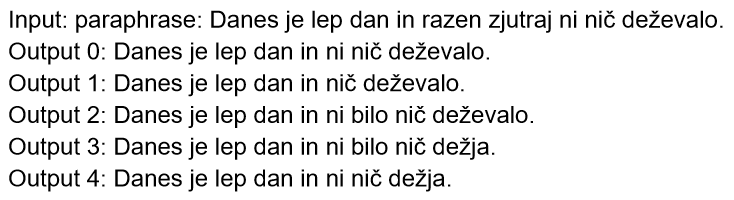
\includegraphics[width=0.9\columnwidth]{NLP_LaTeX_Template/fig/outputs/LepDan.png}
    \caption{Input and 5 different outputs of our model. }
    \label{fig:output1}
\end{figure}

\begin{figure}[H]
    \centering
    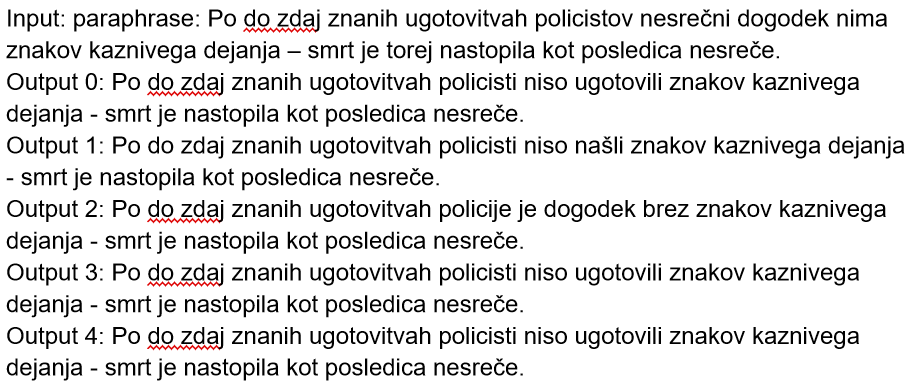
\includegraphics[width=0.9\columnwidth]{NLP_LaTeX_Template/fig/outputs/Obdukcija.png}
    \caption{Input and 5 different outputs of our model. }
    \label{fig:output2}
\end{figure}


\begin{figure}[H]
    \centering
    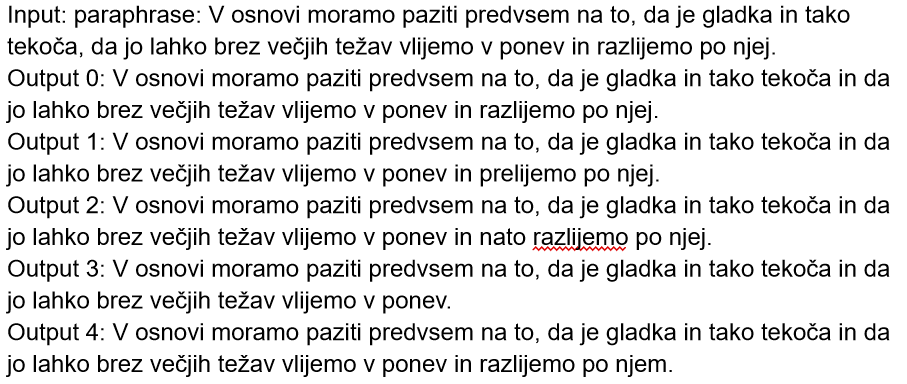
\includegraphics[width=0.9\columnwidth]{NLP_LaTeX_Template/fig/outputs/palačinke.png}
    \caption{Input and 5 different outputs of our model. }
    \label{fig:output3}
\end{figure}


\begin{figure}[H]
    \centering
    \includegraphics[width=0.9\columnwidth]{NLP_LaTeX_Template/fig/outputs/Onesnaževanje.png}
    \caption{Input and 5 different outputs of our model. }
    \label{fig:output4}
\end{figure}

% ROUGE-N and ROUGE-L are mostly used.

%\section*{Methods}


% Use the Methods section to describe what you did an how you did it -- in what way did you prepare the data, what algorithms did you use, how did you test various solutions ... Provide all the required details for a reproduction of your work.

% Below are \LaTeX examples of some common elements that you will probably need when writing your report (e.g. figures, equations, lists, cod e examples ...).


% \subsection*{Equations}

% You can write equations inline, e.g. $\cos\pi=-1$, $E = m \cdot c^2$ and $\alpha$, or you can include them as separate objects. The Bayes’s rule is stated mathematically as:

% \begin{equation}
% 	P(A|B) = \frac{P(B|A)P(A)}{P(B)},
% 	\label{eq:bayes}
% \end{equation}

% where $A$ and $B$ are some events. You can also reference it -- the equation \ref{eq:bayes} describes the Bayes's rule.

% \subsection*{Lists}

% We can insert numbered and bullet lists:

% % the [noitemsep] option makes the list more compact
% \begin{enumerate}[noitemsep] 
% 	\item First item in the list.
% 	\item Second item in the list.
% 	\item Third item in the list.
% \end{enumerate}

% \begin{itemize}[noitemsep] 
% 	\item First item in the list.
% 	\item Second item in the list.
% 	\item Third item in the list.
% \end{itemize}

% We can use the description environment to define or describe key terms and phrases.

% \begin{description}
% 	\item[Word] What is a word?.
% 	\item[Concept] What is a concept?
% 	\item[Idea] What is an idea?
% \end{description}


% \subsection*{Figures}

% You can insert figures that span over the whole page, or over just a single column. The first one, \figurename~\ref{fig:column}, is an example of a figure that spans only across one of the two columns in the report.

% \begin{figure}[ht]\centering
% 	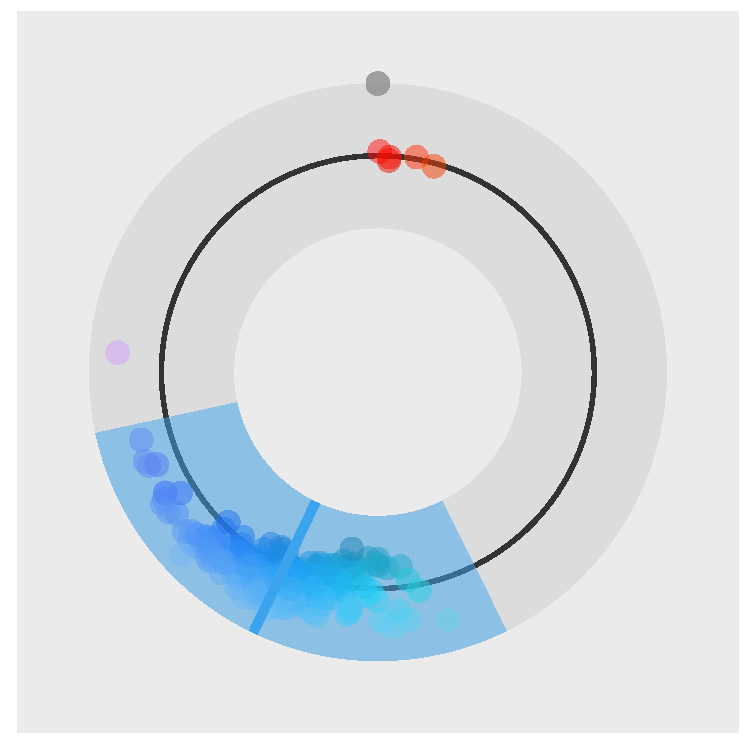
\includegraphics[width=\linewidth]{single_column.pdf}
% 	\caption{\textbf{A random visualization.} This is an example of a figure that spans only across one of the two columns.}
% 	\label{fig:column}
% \end{figure}

% On the other hand, \figurename~\ref{fig:whole} is an example of a figure that spans across the whole page (across both columns) of the report.

% % \begin{figure*} makes the figure take up the entire width of the page
% \begin{figure*}[ht]\centering 
% 	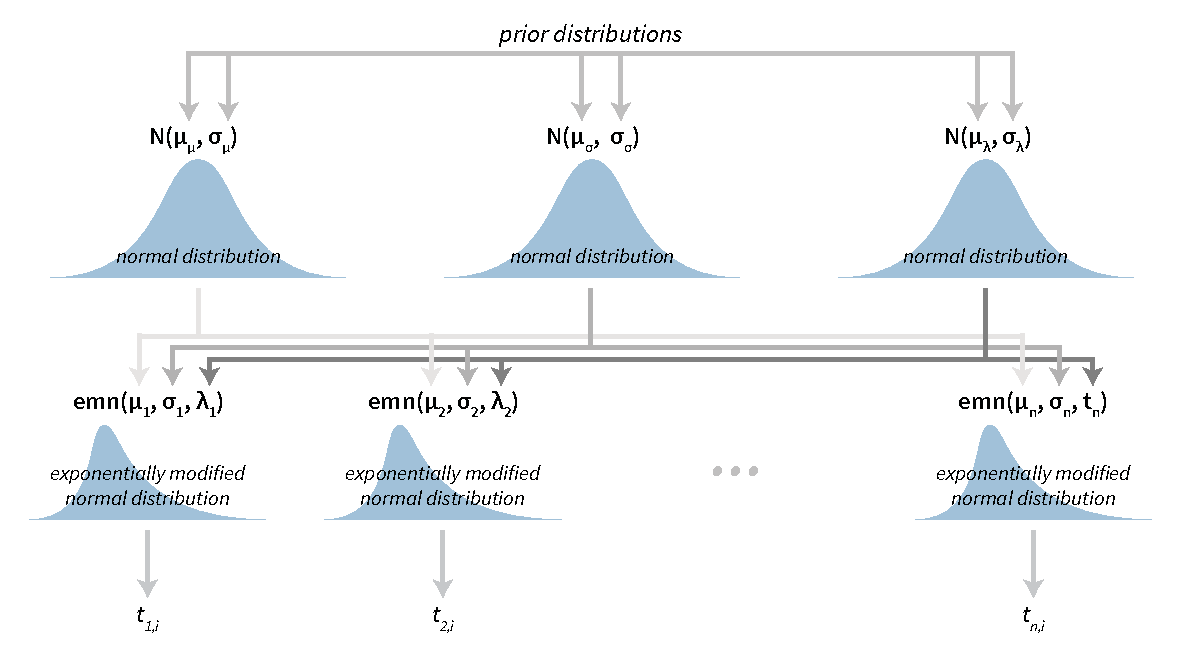
\includegraphics[width=\linewidth]{whole_page.pdf}
% 	\caption{\textbf{Visualization of a Bayesian hierarchical model.} This is an example of a figure that spans the whole width of the report.}
% 	\label{fig:whole}
% \end{figure*}


% \subsection*{Tables}

% Use the table environment to insert tables.

% \begin{table}[hbt]
% 	\caption{Table of grades.}
% 	\centering
% 	\begin{tabular}{l l | r}
% 		\toprule
% 		\multicolumn{2}{c}{Name} \\
% 		\cmidrule(r){1-2}
% 		First name & Last Name & Grade \\
% 		\midrule
% 		John & Doe & $7.5$ \\
% 		Jane & Doe & $10$ \\
% 		Mike & Smith & $8$ \\
% 		\bottomrule
% 	\end{tabular}
% 	\label{tab:label}
% \end{table}


% \subsection*{Code examples}

% You can also insert short code examples. You can specify them manually, or insert a whole file with code. Please avoid inserting long code snippets, advisors will have access to your repositories and can take a look at your code there. If necessary, you can use this technique to insert code (or pseudo code) of short algorithms that are crucial for the understanding of the manuscript.

% \lstset{language=Python}
% \lstset{caption={Insert code directly from a file.}}
% \lstset{label={lst:code_file}}
% \lstinputlisting[language=Python]{code/example.py}

% \lstset{language=R}
% \lstset{caption={Write the code you want to insert.}}
% \lstset{label={lst:code_direct}}
% \begin{lstlisting}
% import(dplyr)
% import(ggplot)

% ggplot(diamonds,
% 	   aes(x=carat, y=price, color=cut)) +
%   geom_point() +
%   geom_smooth()
% \end{lstlisting}

%------------------------------------------------

% \section*{Results}

% Use the results section to present the final results of your work. Present the results in a objective and scientific fashion. Use visualisations to convey your results in a clear and efficient manner. When comparing results between various techniques use appropriate statistical methodology.

% For results we will use different metrics of evaluation. These are BLEU, GLEU, ROUGE, BERTscore, METEOR, WER.


%------------------------------------------------

% \section*{Discussion}

% Use the Discussion section to objectively evaluate your work, do not just put praise on everything you did, be critical and exposes flaws and weaknesses of your solution. You can also explain what you would do differently if you would be able to start again and what upgrades could be done on the project in the future.


%------------------------------------------------

% \section*{Acknowledgments}

% Here you can thank other persons (advisors, colleagues ...) that contributed to the successful completion of your project.


%----------------------------------------------------------------------------------------
%	REFERENCE LIST
%----------------------------------------------------------------------------------------
\bibliographystyle{unsrt}
\bibliography{report}


\end{document}

